\documentclass{beamer}

\usecolortheme[light]{solarized}

\beamertemplatenavigationsymbolsempty
\setbeamertemplate{frametitle}[default][center]

\usepackage{hyperref}
\usepackage{minted}

\usepackage{graphicx}
\usepackage{tikz}

\usetikzlibrary{calc, patterns}

\begin{document}

    \begin{frame}
        \begin{center}
            \Large

            Welcome to Cardiff!

            \vfill
            \begin{center}
                
\includegraphics[width=3cm]{./img/CUident_CMYK.eps}
            \end{center}
            % Bi-lingual country: GP
            % Capital of Wales: VK
            % Dr Who stuff happens here: GP
            % Population of 341,000 (a fifth of which are students): VK
            % The UK's first female professor (of education): Millicent
            % MacKenzie in 1910
            % http://blogs.cardiff.ac.uk/cuarm/millicent-mackenzie/: VK
        \end{center}

    \end{frame}

    \begin{frame}
        \begin{center}
            \fbox{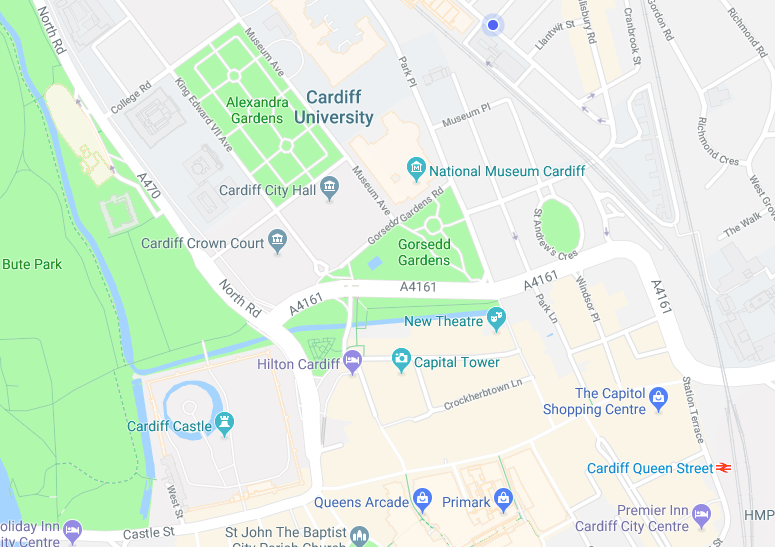
\includegraphics[width=.8\textwidth]{./img/cardiff.png}%: GP
        \end{center}
    \end{frame}

    \begin{frame}
        \begin{center}
            \fbox{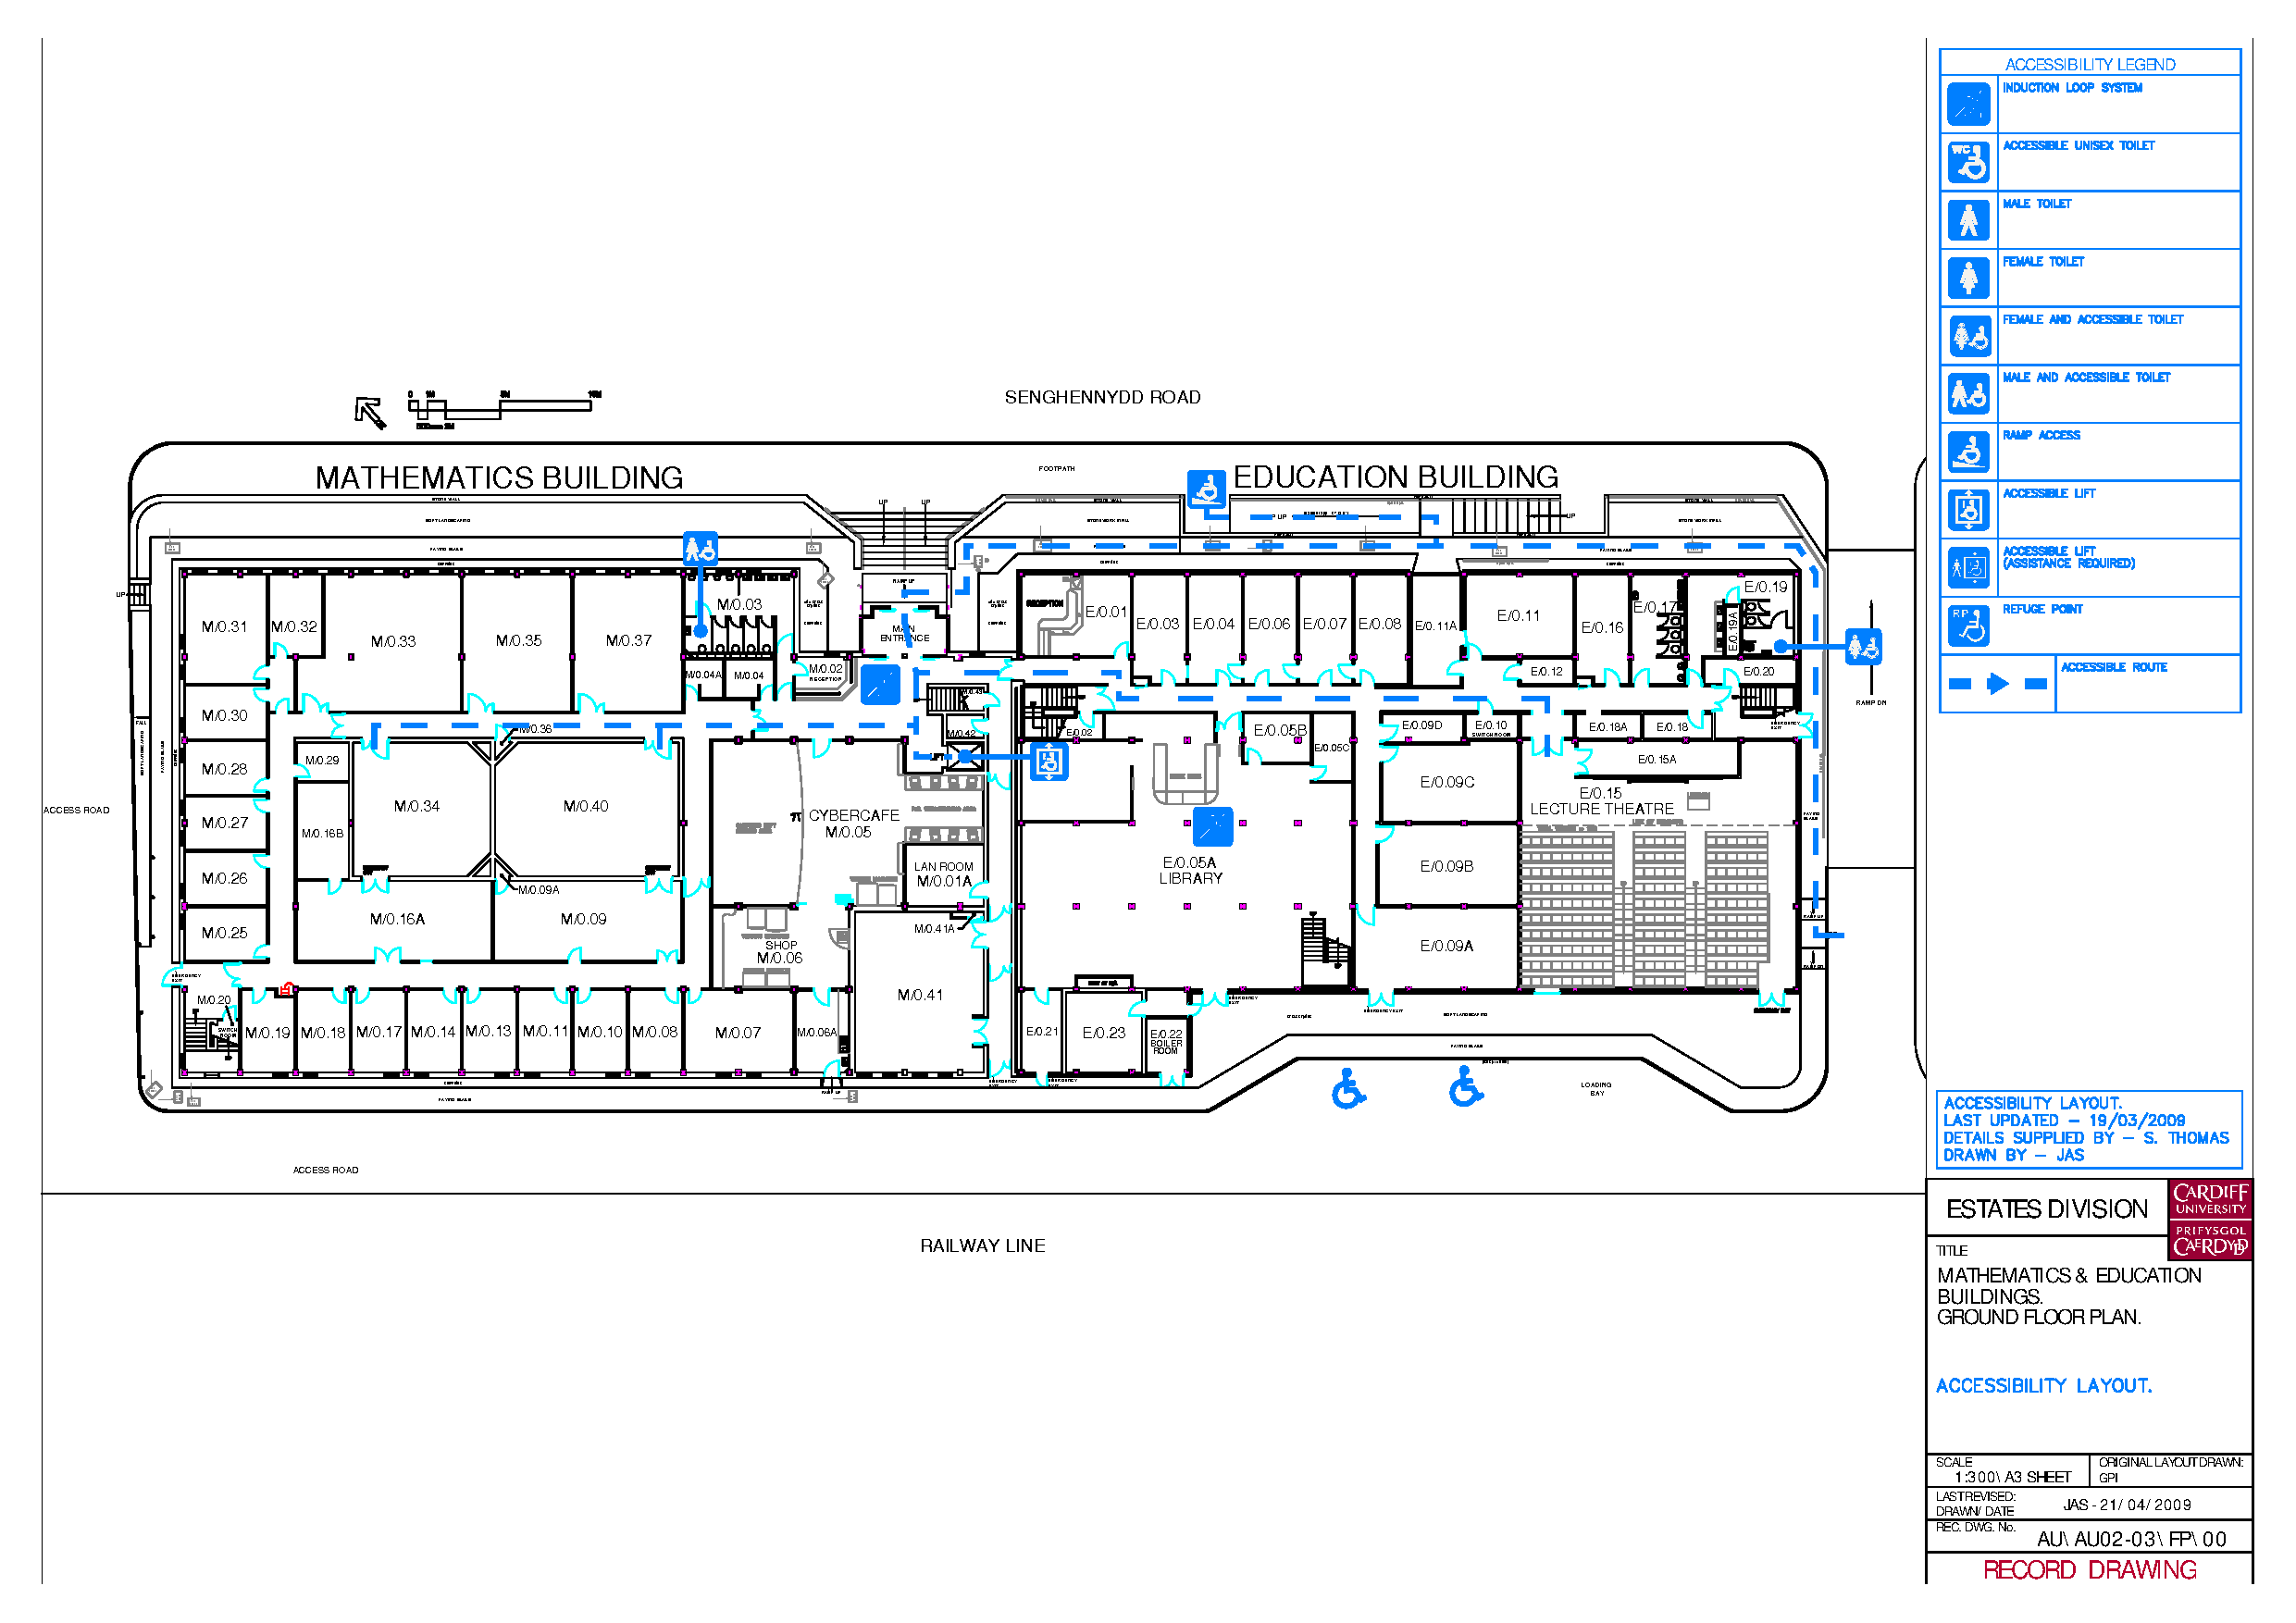
\includegraphics[clip, trim=3cm 6.5cm 7cm 7cm, width=.8\textwidth]{./img/Maths-and-Education-Building-Ground-Floor.pdf}}

            \vfill
            \fbox{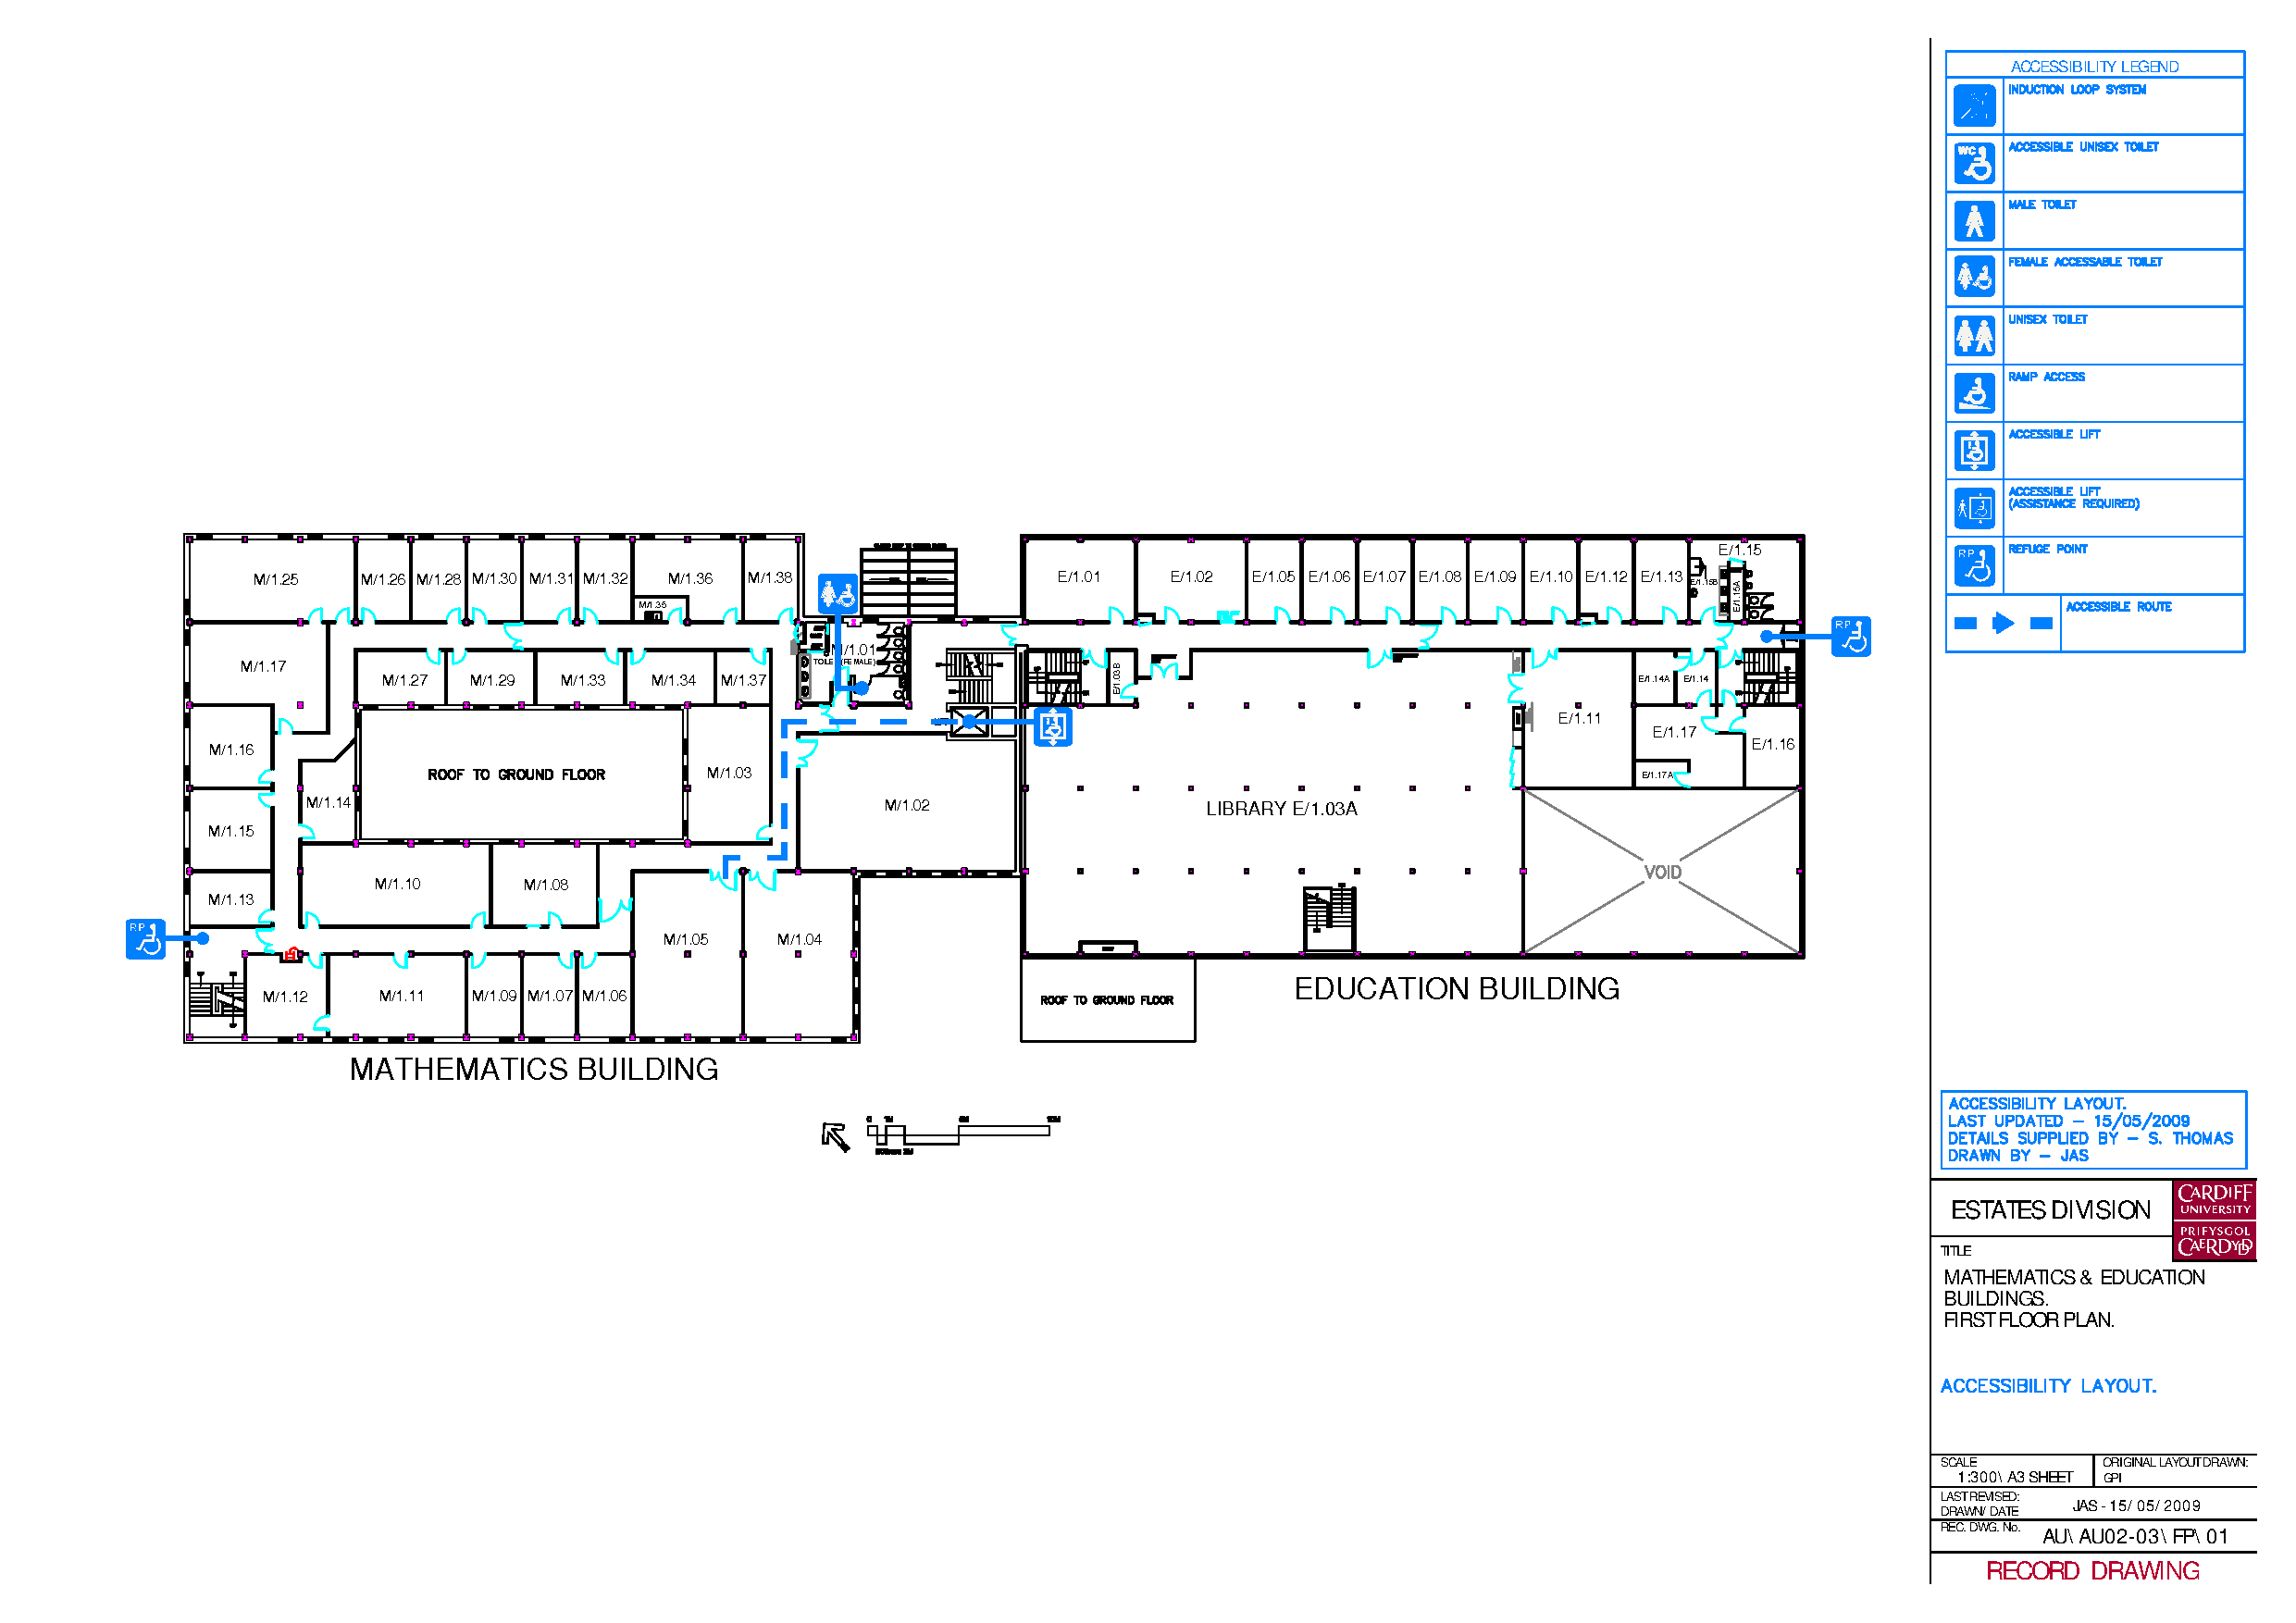
\includegraphics[clip, trim=3cm 8cm 7cm 9cm, width=.8\textwidth]{./img/Maths-and-Education-Building-First-Floor.pdf}}
            % Lifts
            % Bathroom
            % No fire alarms
        \end{center}
    \end{frame}

\end{document}
